% DO NOT COMPILE THIS FILE DIRECTLY!
% This is included by the other .tex files.

\begin{frame}[t,plain]
\titlepage
\end{frame}

\begin{frame}
	\frametitle{This session is meant to answer the following}
	\begin{itemize}
		\item What is Cerebrate?
                \item Why are we working on this?
                \item What sort of benefits does this bring for MISP communities?
                \item What is there and where are we headed?
	\end{itemize}
\end{frame}

\begin{frame}
	\frametitle{What is Cerebrate?}
	\begin{itemize}
                \item Open source {\bf community management and orchestration} tool
                \item Central tool for the Melicertes 2 project
                \item Tight integration with various open-source tools
                \item Planned as the primary MISP management tool
                \item Test bed for the new tech stack and a host of new features coming to MISP
	\end{itemize}
\end{frame}

\begin{frame}
	\frametitle{What issues is it trying to tackle?}
	\begin{itemize}
                \item Community management
		\begin{itemize}
                    \item {\bf Repository} of organisations and individuals
                    \item Management of {\bf sharing groups}
                    \item {\bf Exchange} of contact and sharing group information
                    \item Cryptographic key lookup for {\bf information signing}
		\end{itemize}
                \item Local tool management
		\begin{itemize}
                    \item Instrumentation of {\bf local tool interconnections}
                    \item Local tool {\bf fleet management}
                    \item {\bf Feeding} the local tools with Cerebrate data
                \end{itemize}
	\end{itemize}
\end{frame}

\begin{frame}
	\frametitle{What is available currently?}
	\begin{itemize}
                \item {\bf ContactDB}
                \item {\bf Sharing group management}
                \item {\bf Cerebrate to Cerebrate synchronisation}
                \item Local tool orchestration - {\bf integration modules}
                \item {\bf Inbox} system
                \item Local tool {\bf fleet management}
                \item {\bf Update} management
	\end{itemize}
\end{frame}

\begin{frame}
\frametitle{ContactDB}
\begin{center}
    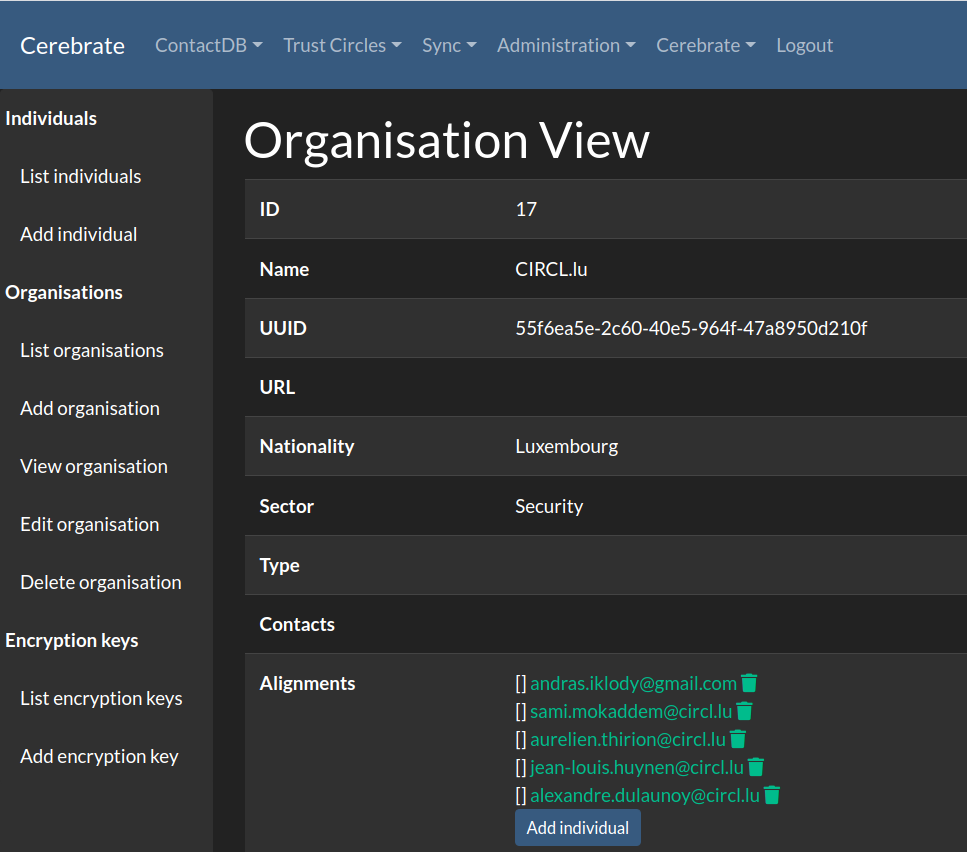
\includegraphics[scale=0.4]{org.png}
\end{center}
\end{frame}


\begin{frame}
\frametitle{Sharing groups}
\begin{center}
    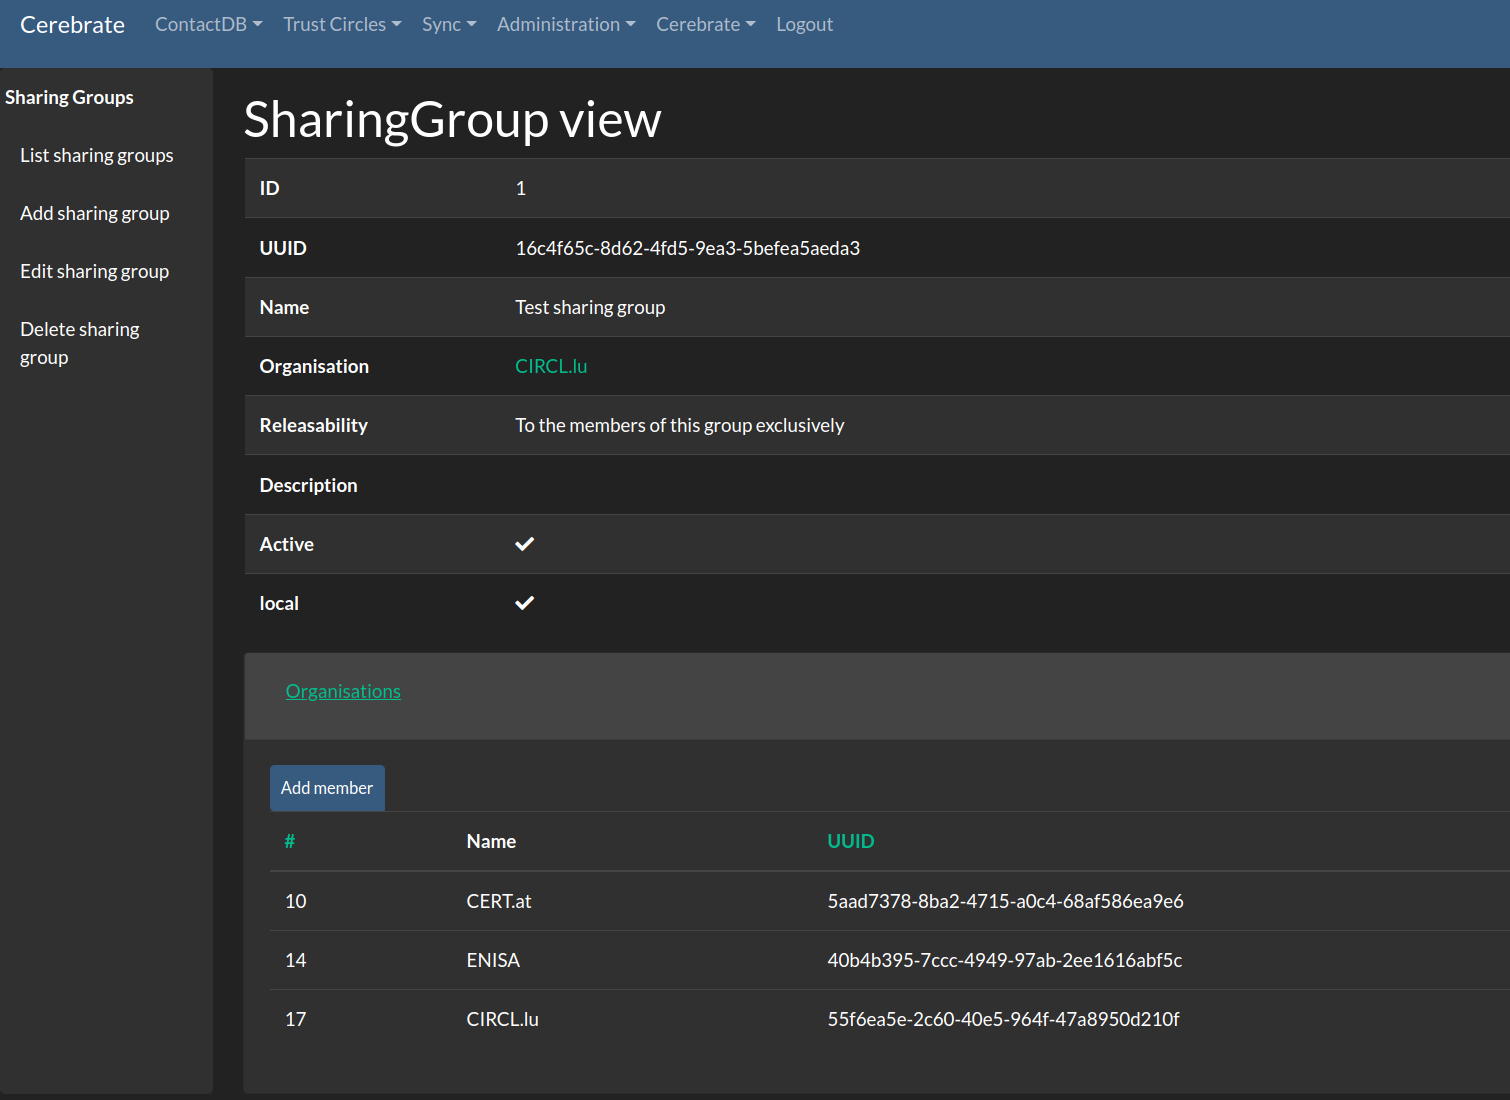
\includegraphics[scale=0.25]{sharing_group.png}
\end{center}
\end{frame}

\begin{frame}
\frametitle{Bigger picture}
\begin{center}
    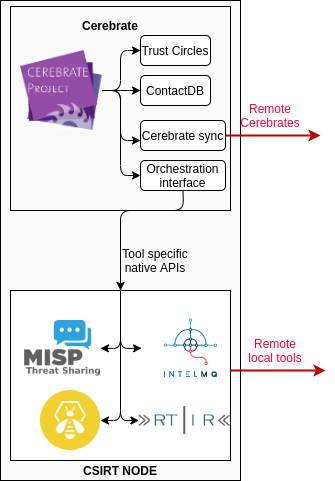
\includegraphics[scale=0.4]{Goals.png}
\end{center}
\end{frame}

\begin{frame}
\frametitle{Synchronisation}
\begin{center}
    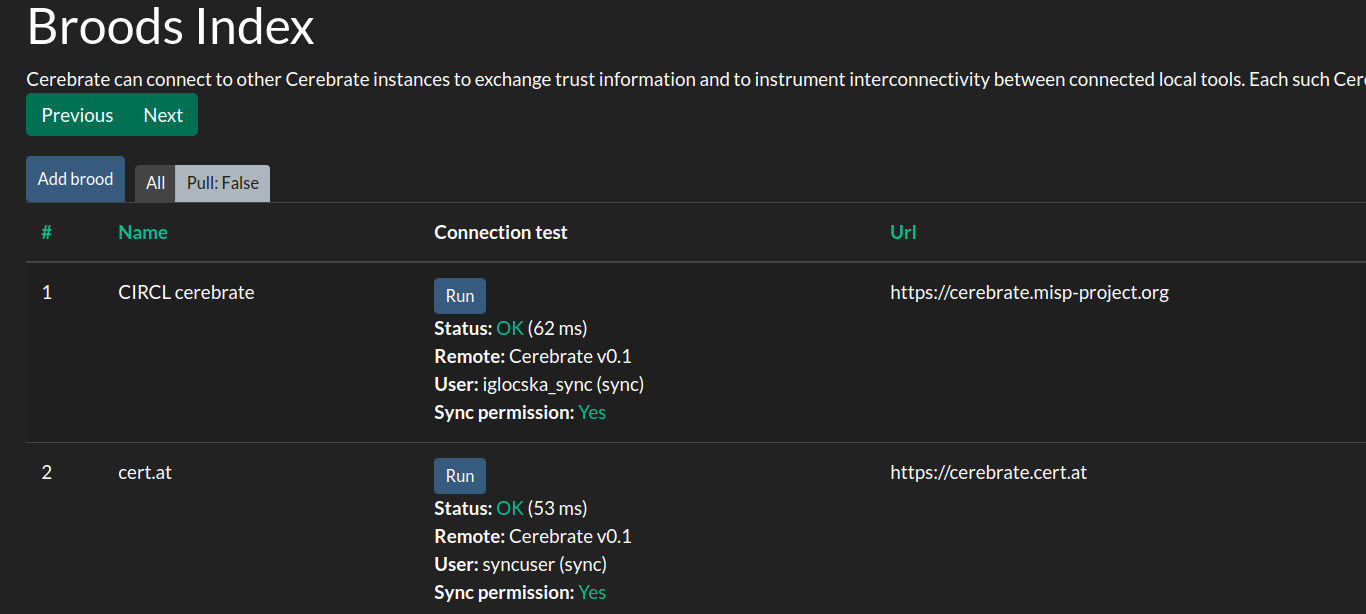
\includegraphics[scale=0.4]{sync.png}
\end{center}
\end{frame}

\begin{frame}
	\frametitle{Synchronisation}
	\begin{itemize}
                \item {\bf Connect} Cerebrates to one another
                \item {\bf Diagnose} connectivity issues
                \item Remotely {\bf browse the data} of the remote instance
                \item {\bf Fetch} organisation, individual, sharing group data
	\end{itemize}
\end{frame}

\begin{frame}
	\frametitle{Integration modules}
	\begin{itemize}
                \item Tool agnostic integration layer
                \item Integrate other tools with Cerebrate for a set of tasks
         	\begin{itemize}
		        \item {\bf Manage} tools
		        \item {\bf Feed} the tool with / feed off the tool's contact information
                        \item {\bf Orchestrate} the {\bf interconnection} between local tools
                        \item Open a {\bf dialogue} with partners to interconnect tools
		\end{itemize}
	\end{itemize}
\end{frame}

\begin{frame}
\frametitle{Local tools and contactDB, SGs}
\begin{center}
    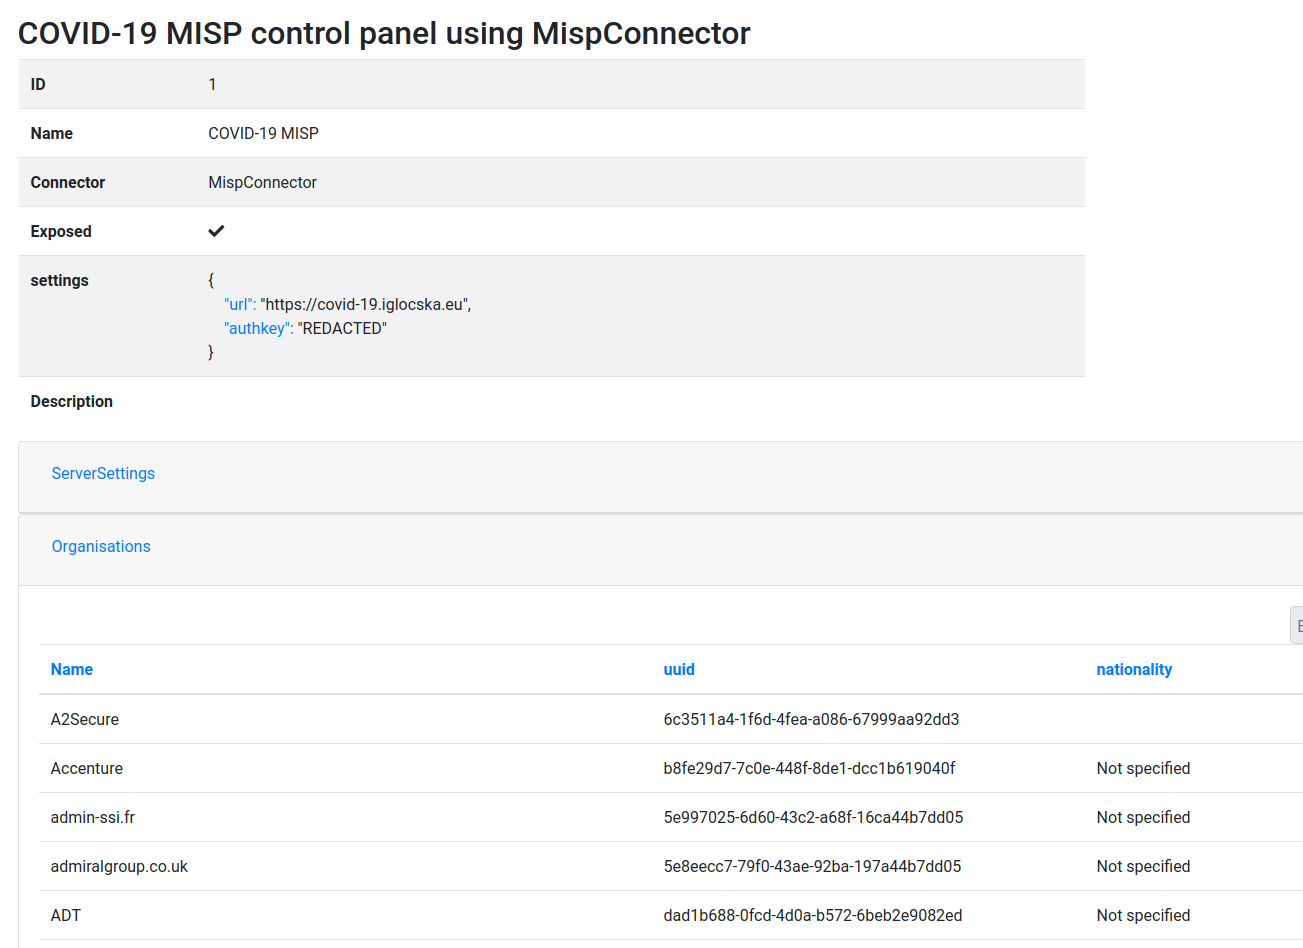
\includegraphics[scale=0.28]{misp_orgs.png}
\end{center}
\end{frame}

\begin{frame}
\frametitle{Fleet management}
\begin{center}
    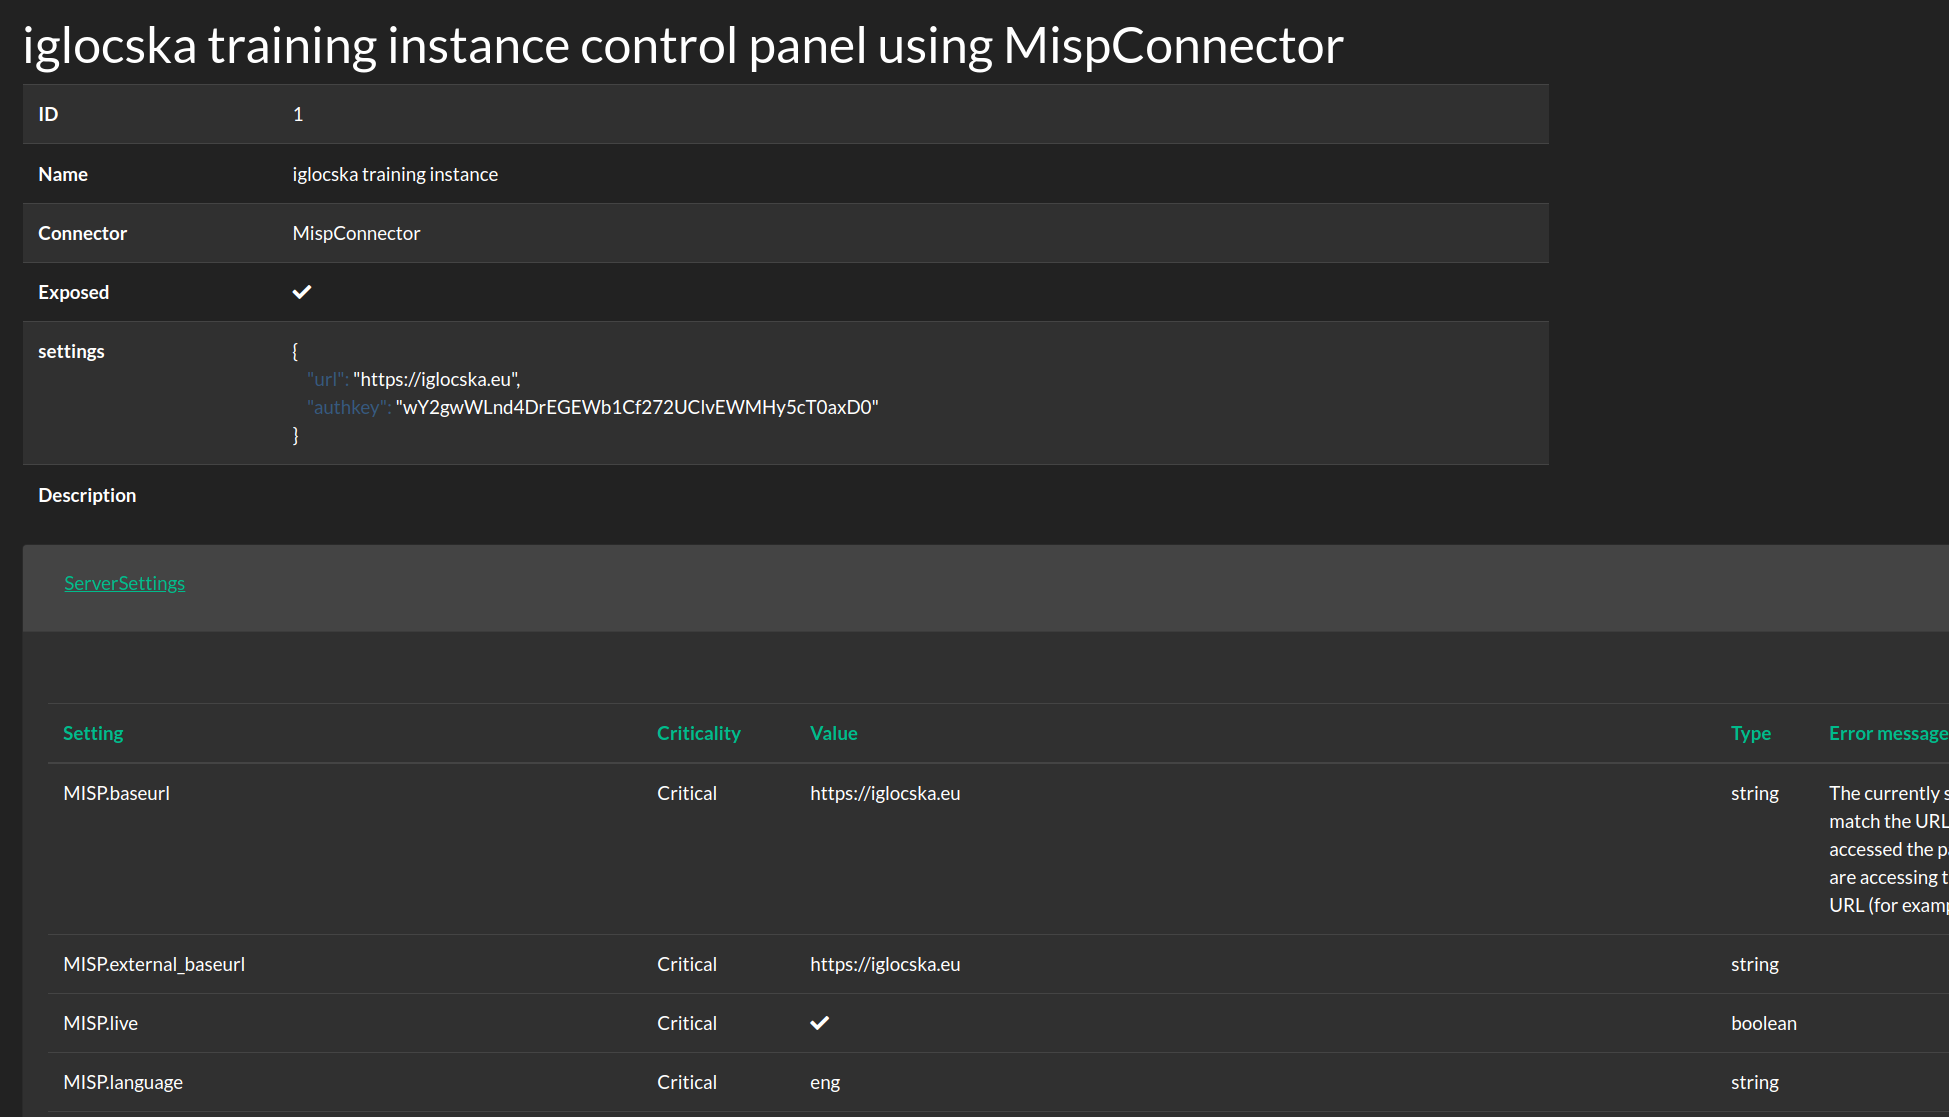
\includegraphics[scale=0.25]{local_tool_settings.png}
\end{center}
\end{frame}


\begin{frame}
\frametitle{Interconnect tools}
\begin{center}
    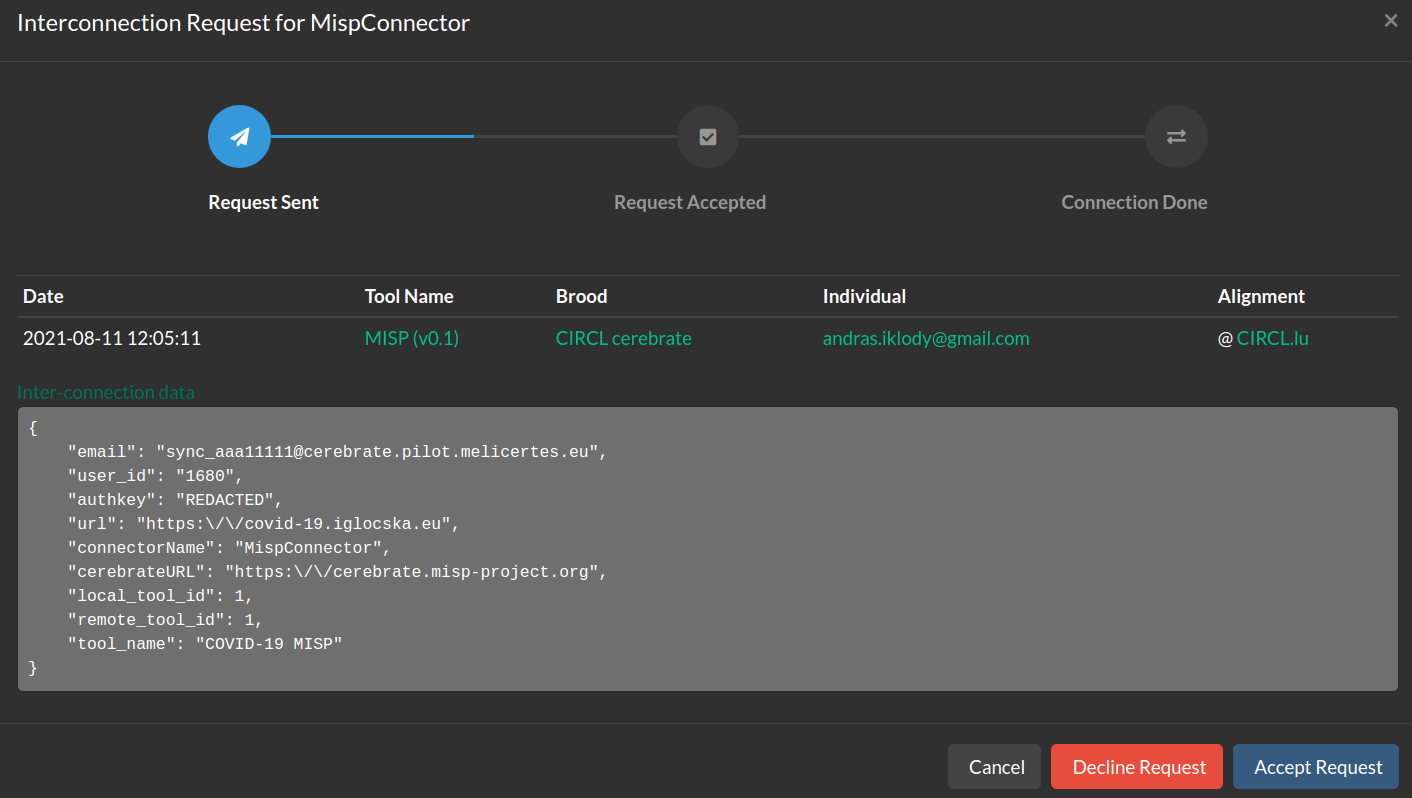
\includegraphics[scale=0.3]{interconnection.png}
\end{center}
\end{frame}


\begin{frame}
	\frametitle{Update management}
	\begin{itemize}
                \item Manage the {\bf updating} of Cerebrate's {\bf database} directly from the UI / API
                \item Part of the new patch management system
                \item Review the {\bf state of the patches and potential failures}
                \item This will also be the future update management tool of MISP
	\end{itemize}
\end{frame}

\begin{frame}
\frametitle{Update management}
\begin{center}
    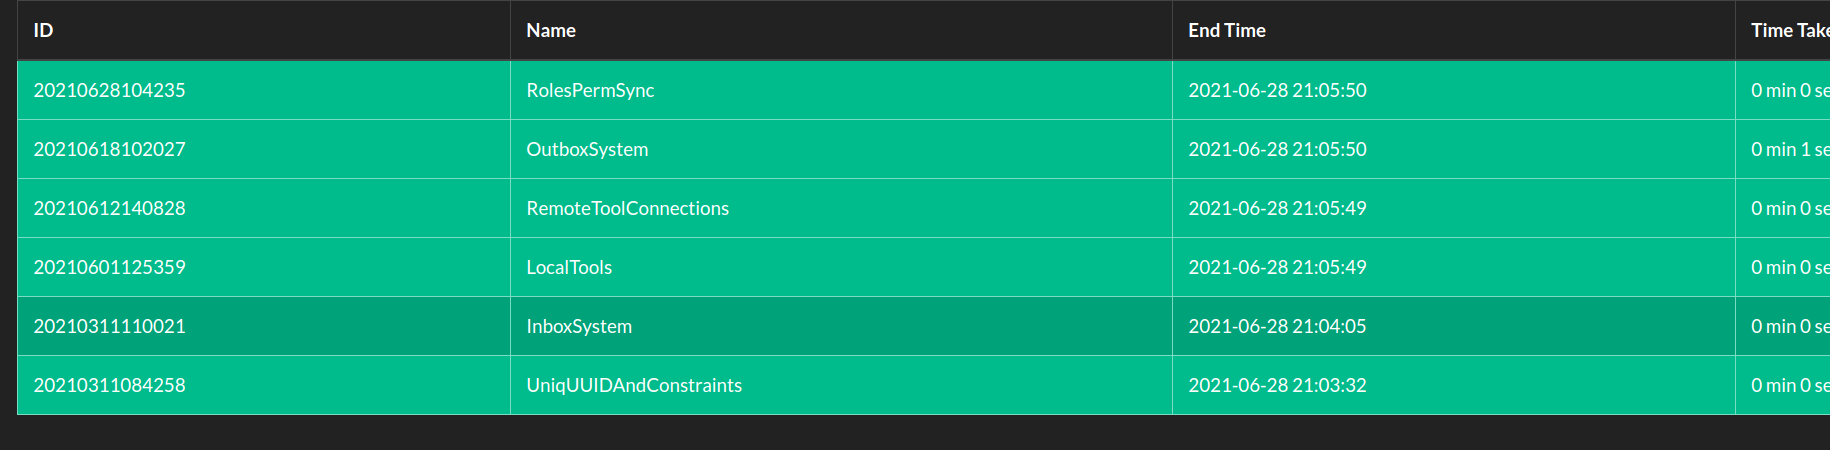
\includegraphics[scale=0.3]{updates.png}
\end{center}
\end{frame}

\begin{frame}
	\frametitle{Configuration system}
	\begin{itemize}
                \item It is currently in testing / finalisation phase
                \item Configure and {\bf manage} your Cerebrate instance via the {\bf UI / API}
                \item Look and feel, security, features all configurable
                \item This will also {\bf replace MISP's configuration and diagnostics} system in the future
	\end{itemize}
\end{frame}

\begin{frame}
\frametitle{Configuration system}
\begin{center}
    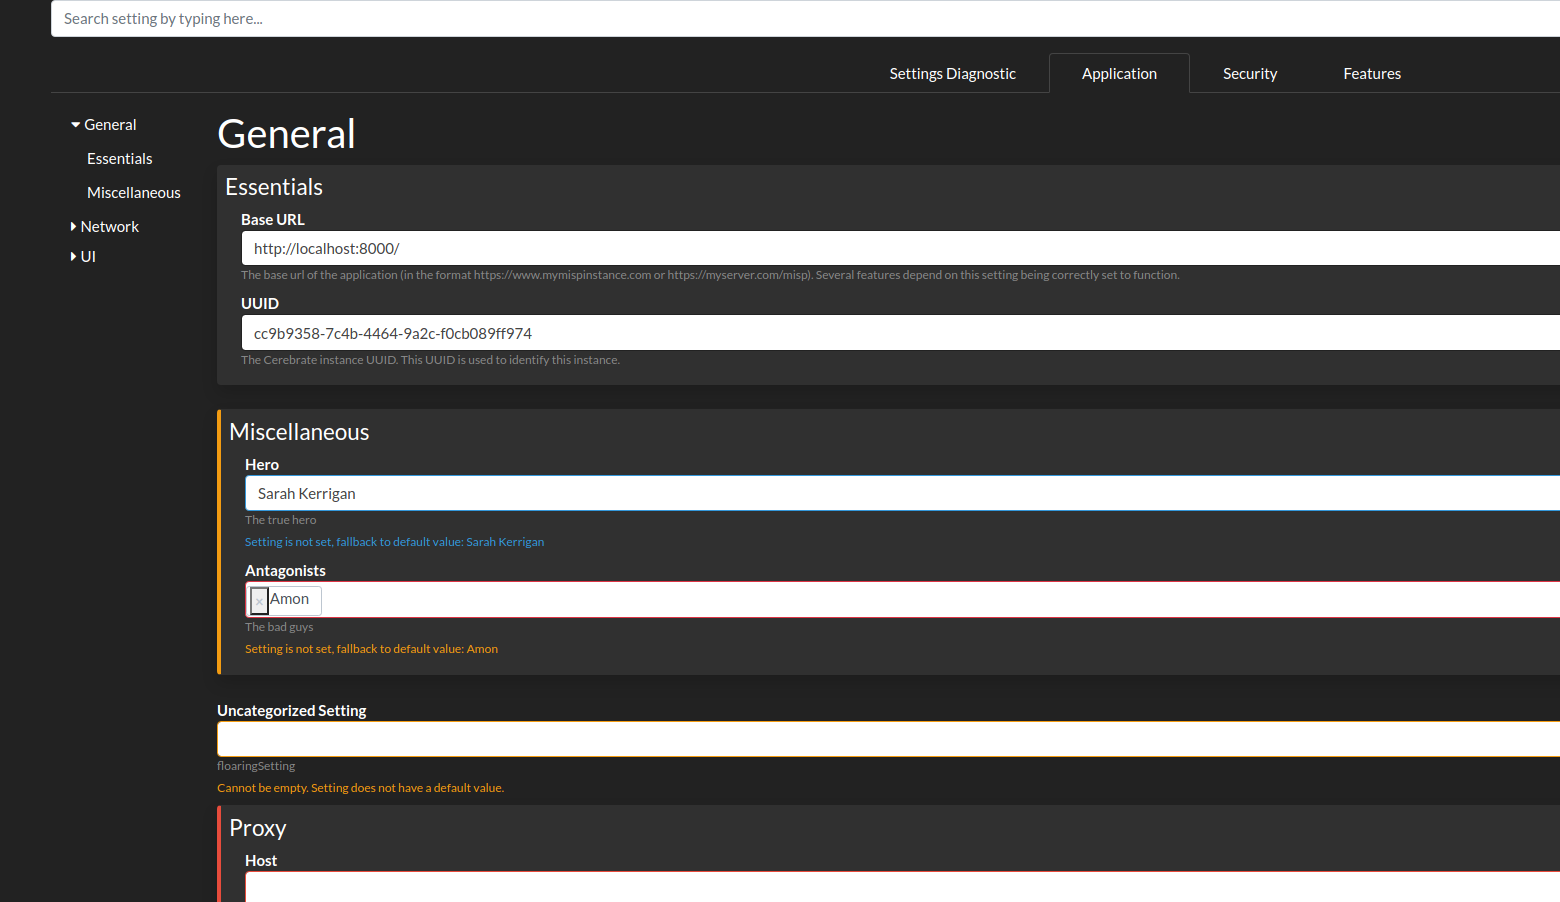
\includegraphics[scale=0.3]{config.png}
\end{center}
\end{frame}

\begin{frame}
	\frametitle{What are we working on?}
	\begin{itemize}
                \item Obviously moving MISP to the same feature-set / tech stack
                \item Further integrations with other tools
                \item Fleshing out the MISP monitoring and management
                \item Integrating Cerebrate (and later MISP) with IAM systems
                \item Setting up trusted, community centric Cerebrate nodes
	\end{itemize}
\end{frame}
